\subsection{Dreamfusion}\label{dreamfusion}

DreamFusion, as introduced by \citeauthor{pooleDreamfusion}, marks a significant advancement in the field of 3D modeling. Utilizing Neural Radiance Fields (NeRF), DreamFusion employs a novel technique known as Score Distillation Sampling (SDS) to generate coherent 3D objects and scenes from a variety of text prompts. This approach diverges from traditional methods that depend on pre-existing images from multiple angles, as DreamFusion dynamically generates these images during training using a diffusion model.

Central to DreamFusion is the use of Differentiable Image Parameterization (DIP), as described by \citep{mordvintsevDIP}. This technique enables the generation of images \( x \) through parameters \( \theta \) and a differentiable generator \( g \), offering refined optimization capabilities even at the pixel level \citep{pooleDreamfusion}. This marks a shift from the conventional approach of diffusion models, which usually produce outputs similar to their training data. In DreamFusion, the parameters \( \theta \) define 3D volumes, with \( g \) functioning as a volumetric renderer. 

In the Score Distillation Sampling (SDS) method, the initial step involves identifying the best parameters \( \theta \) for the model \(\phi\). This involves minimizing the loss in relation to a datapoint created by a model.~\citeauthor{pooleDreamfusion} use the formular~\[ \theta^{*} = \text{arg min}_{\theta} \mathcal{L}_{\text{Diff}}(\phi, \mathbf{x} = g(\theta)) \] This essentially means the model is adjusted to find the parameters \( \theta \) that bring its output as close as possible to the desired result based on textual input. The primary SDS function by \citeauthor{pooleDreamfusion} is:~\[
\nabla_{\theta}\mathcal{L}_{\text{SDS}}(\phi,\mathbf{x}=g(\theta))\triangleq\mathbb{E}_{t,\epsilon}\left[w(t)\left(\hat{\epsilon}_{\phi}({\mathbf{z}}_{t};y,t)-\epsilon\right){\frac{\partial\mathbf{x}}{\partial\theta}}\right]
\] In this equation, \( w(t) \) acts as a weighting factor, modifying the influence of different components within the formula. The term \( \hat{\epsilon}_{\phi}({\mathbf{z}}_{t};y,t) \) represents the score function predicted by the diffusion model \( \phi \). This function estimates the noise adjustments needed based on the noisy image \( z_t \), the text embedding \( y \), and the noise level \( t \). The actual noise at time \( t \) is denoted by \( \epsilon \). This function is key in determining how the noise should be adjusted during the diffusion process to align the generated image with the text input. Additionally, the term \( \frac{\partial\mathbf{x}}{\partial\theta} \) indicates how changes in the model’s parameters \( \theta \) affect the image \( \mathbf{x} \), guiding the optimization process. SDS adds controlled noise to an image \( x \) at each timestep \( t \), and then adjusts it based on the model's scoring, efficiently updating the image to closely match the text descriptions without the need for traditional backpropagation \citep{pooleDreamfusion}.

\begin{figure}[ht]
  \centering
    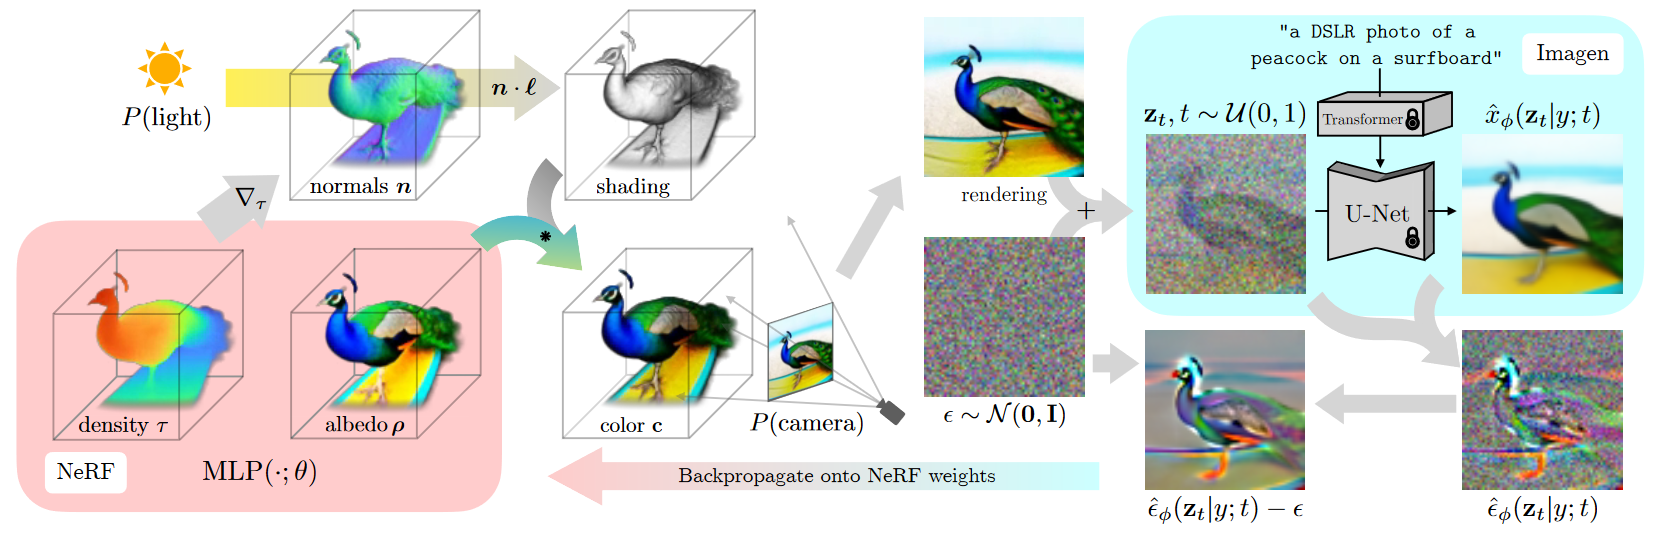
\includegraphics[width=1\columnwidth]{figures/Dreamfusion.png}
    \caption{Summatized functionality of Dreamfusion, image by \citep{pooleDreamfusion}}\label{fig:figureDreamfusion}
  \end{figure}

DreamFusion offers an innovative approach to transforming text into 3D models, as depicted in Figure~\ref{fig:figureDreamfusion}. This process employs several key components: natural language captions for directional guidance, Google's Imagen as the text-to-image diffusion model \citep{saharia2022imagen}, an imporved version of Neural Radiance Field, the mip-NeRF 360 \citep{barron2022mipnerf} ``that reduces aliasing'' \citep{pooleDreamfusion}, and the Score Distillation Sampling (SDS) for the loss function.

At the center of the rendering process is the Neural Radiation Field, which is represented as \( \text{MLP}(\cdot; \theta) \), where the dot \(\cdot\) denotes the input of 3D coordinates and viewing directions. This input is important to determine how light and color interact in 3D space.~\(\theta\) symbolizes the parameters or weights of the MLP that are fine-tuned during training. These parameters determine how the MLP interprets its input (the 3D coordinates and viewing directions) to produce the final output, such as the color and density at each point in the 3D model.

The creation of 3D scenes begins with this parameterization of the NeRF MLP, followed by randomly choosing camera angles and point light positions. This randomness ensures realistic representations from various perspectives \citep{pooleDreamfusion}. Shading plays a crucial role in adding depth and realism, driven by the interaction of light with surface normals, computed from the density gradients and the light position \( l \). Additionally, the inherent color of objects, or albedo, is generated during the NeRF rendering phase. By combining this albedo with the effects of shading, the NeRF accurately renders the final color for each scene point. The result is a detailed visual representation from the selected viewpoint.

After rendering, DreamFusion evaluates the scene against the diffusion model's predictions, assessing diffusion loss to evaluate the match with the expected outcome. The rendered image is then diffused and reconstructed using a static conditional Imagen model, which adds predicted noise \( \hat{\epsilon}_\phi(z_t | y; t) \) into the rendering, to improve fidelity but also increasing variance \citep{pooleDreamfusion}.

The model refinement phase involves subtracting this predicted noise, resulting in a direction with reduced variance. This direction informs the backpropagation through the rendering process, crucial for updating the NeRF's MLP parameters in a manner that more accurately reflects the scene described by the text.

Despite DreamFusion's promising results, it is not without limitations. The model tends to exhibit a lower level of detail, partly due to its reliance on a \( 64 \times 64 \) image model. Furthermore, while SDS is an effective loss function, it sometimes leads to ``oversaturated and oversmoothed results \([\ldots]\)'' \citep{pooleDreamfusion}. Another aspect to consider with SDS is the mode-seeking behavior, which potentially limits the variety of results generated. This limitation is strengthened by the use of KL divergence, ``which has been previously noted to have mode-seeking properties in the context of variational inference and probability density distilaltion''\citep{pooleDreamfusion}. This tendency of the model to prioritize the most frequent patterns can lead to a trade-off between accuracy and diversity, so ``it may be unclear if minimizing this loss will produce good samples'' \citep{pooleDreamfusion}. This statement highlights a major challenge in machine learning, especially with generative models such as DreamFusion. Minimizing loss, a standard method for improving model performance, does not always lead to high-quality or diverse results. There is a risk of overfitting, where the model can reproduce the training data very well, but is less able to generate new and diverse results.